\documentclass[10pt,handout]{beamer}
\usetheme{Rochester}
\usepackage[utf8]{inputenc}
\usepackage{amsmath}
\usepackage{amsfonts}
\usepackage{amssymb}
%\setbeamertemplate{frametitle}[default][center]
\setbeamercolor{page number in head/foot}{fg=black}
\setbeamerfont{page number in head/foot}{size=\small}
\usepackage{xcolor}
\setbeamertemplate{footline}[page number]
%\beamertemplatenavigationsymbolsempty
%\setbeamertemplate{footline}[page number]
%\setbeamertemplate{footline}[frame number]
%\usepackage{siunitx}
\author{Justin Anguiano, Margaret Lazarovitz}
\title{\textcolor{red}{Classifying Charged Particles} from High Energy Collisions at the \textcolor{red}{L}arge \textcolor{red}{H}adron \textcolor{red}{C}ollider }


%\setbeamercovered{transparent} 
%\setbeamertemplate{navigation symbols}{} 
%\logo{} 
\institute{University of Kansas} 
\date{\today} 
%\subject{} 
\begin{document}

\begin{frame}
\titlepage
\end{frame}



\begin{frame}{Introduction}
Overall project goal:\\
\quad \quad \\
\begin{itemize}
\item[] Classify particles better to assist with search for particle
 darkmatter
\item[] \quad
\end{itemize}
Specific focus:
 \begin{itemize}
	
	\item[] \quad
	\item[-] Discrminate low momentum true muons($\mu^\pm$) from particles imitating muons in reconstruction
\end{itemize}


\end{frame}

\begin{frame}{Motivation}
\textbf{KU CMS analysis in progress} -- \textcolor{red}{searching for particle dark matter via compressed SUSY models}\\

\begin{columns}
\begin{column}{0.5\textwidth}
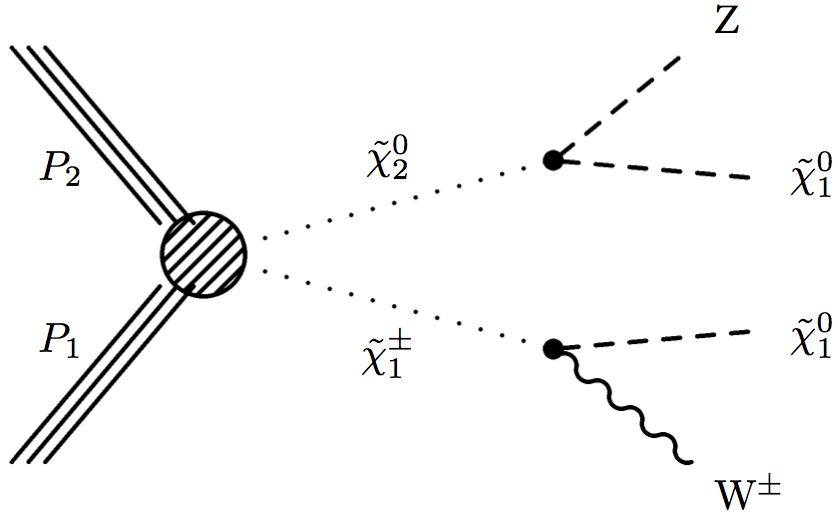
\includegraphics[scale=.75]{TChiWZ.png}
\end{column}
\begin{column}{0.5\textwidth}
\begin{itemize}
\small
\item Protons $P_1$, $P_2$ collide producing SUSY $\tilde \chi^{\pm}_1$,$\tilde \chi_2$ 
\item SUSY $\tilde \chi^{\pm}_1$,$\tilde \chi_2$ decays to D.M. $\tilde \chi^0_1$ and known particles $W^\pm$,$Z$
\item $W^\pm$,$Z$ immediately decay into charged particles($\mu^\pm$) that we see in the detector
\end{itemize}
\end{column}
\end{columns}
\small
\quad \quad \\
A compressed scenario implies $\tilde \chi^{\pm}_1$,$\tilde \chi_2$ and  $\tilde \chi^0_1$ are very close in rest mass\\
\quad \quad \\
With compression the decay products of $\tilde \chi^{\pm}_1$,$\tilde \chi_2$ are soft (low momentum), including ending charged particles\\
\quad \quad \\
The current CMS detector is less optimized for correctly identifying soft $\mu^\pm$\\
\quad \quad \\
If we can optimize soft charged particle classification, we have a better chance of discovering compressed $\tilde \chi^{\pm}_1$,$\tilde \chi_2$, and $\tilde \chi^0_1$

\end{frame}

\begin{frame}{Anatomy of an Event}
\begin{columns}
\begin{column}{0.5\textwidth}
The ``physics workflow" 
\begin{itemize}
\small
\item An event consists of \textcolor{red}{colliding protons} which \textcolor{red}{produces particles} showering outward(transverse)\\

\item We \textcolor{red}{measure the energy and momentum} of all the visible particles in the event

\item There are 100s of charged particles per event\\

\item \textcolor{red}{Reconstruct intermediate or invisible particles} through momentum and energy conservation
\end{itemize}

\end{column}
\begin{column}{0.5\textwidth}
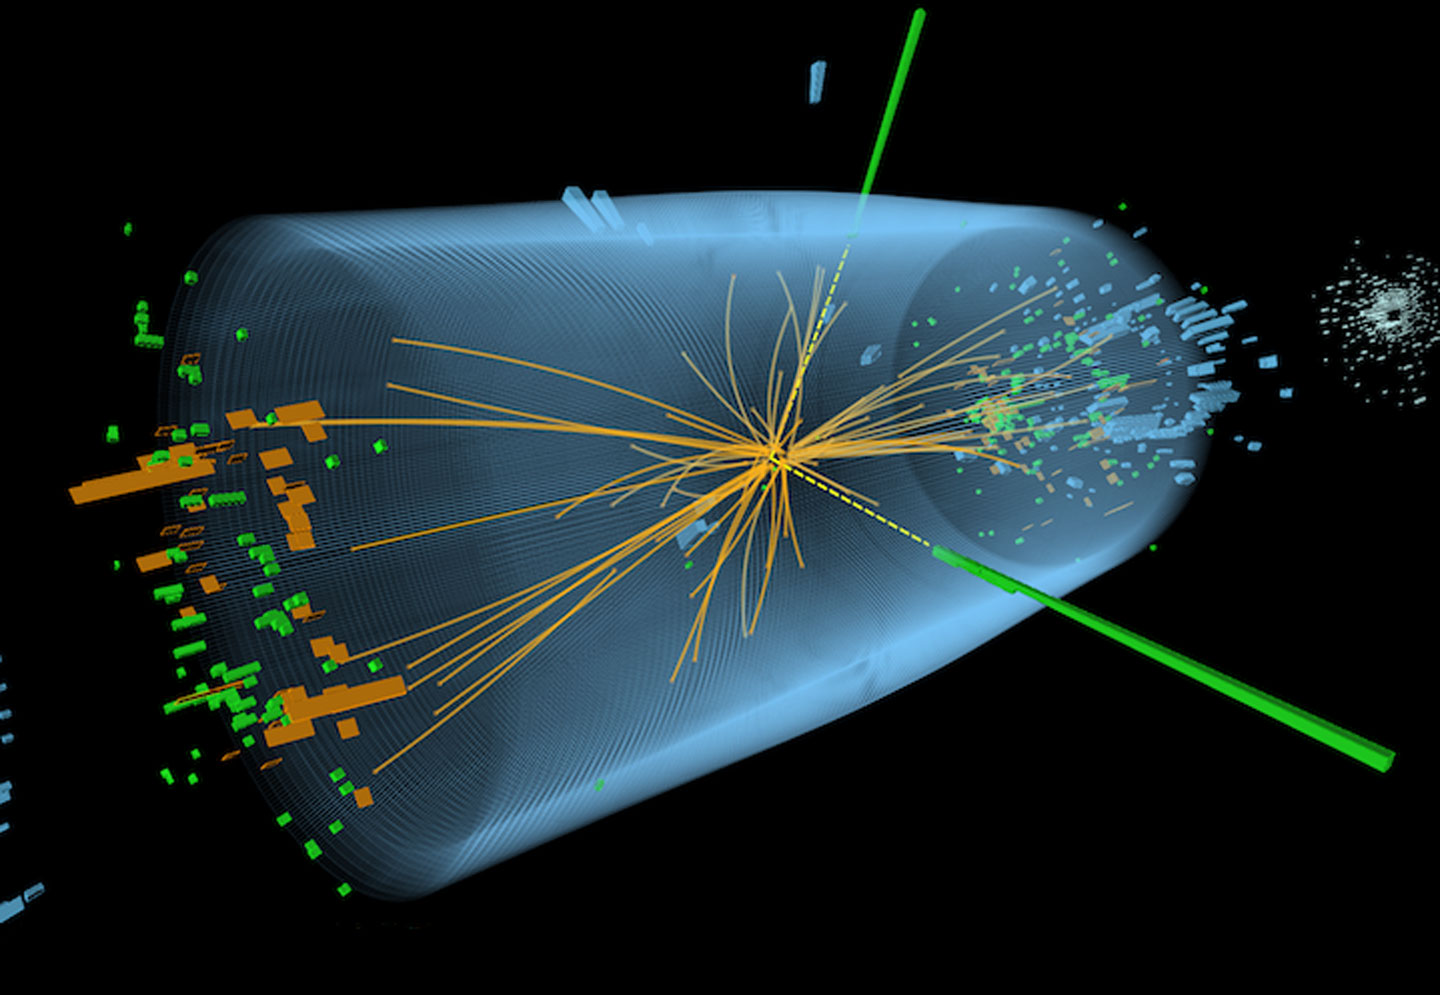
\includegraphics[scale=.12]{cms-event.jpg}\\
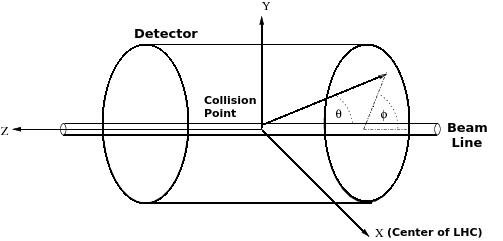
\includegraphics[scale=.2]{coords.png}
\end{column}
\end{columns}



\end{frame}

\begin{frame}{Charged Particle Reconstruction}
\begin{columns}
\begin{column}{0.5\textwidth}
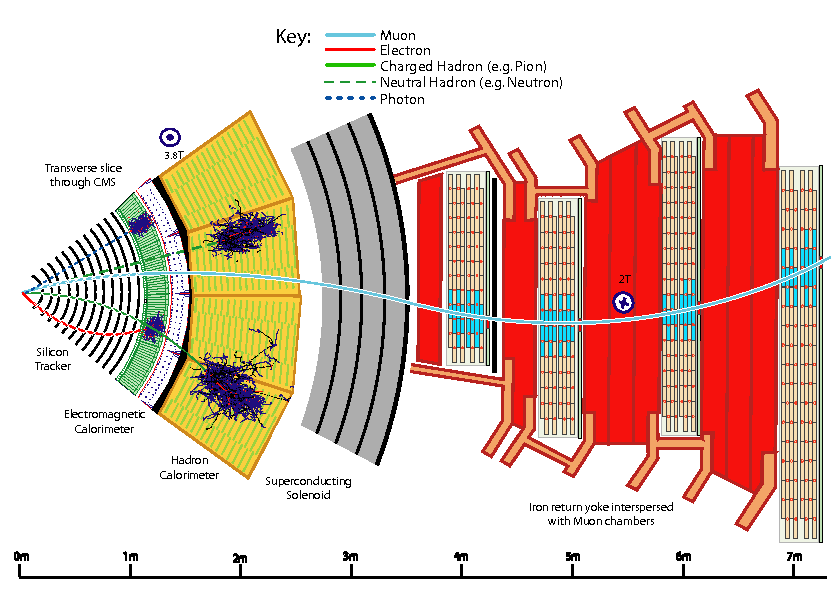
\includegraphics[scale=0.2]{particles.png}\\
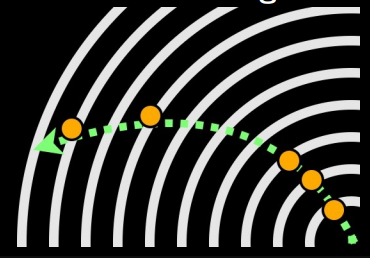
\includegraphics[scale=0.2]{trackreco.png}
\end{column}
\begin{column}{0.5\textwidth}
\small
Charged particles bend in Mag. field and create ``tracks"\\
\quad \quad \\
Tracks are connecting the dots: ``hits'' that are fit with a curve \\
\quad \quad \\
Main particle of interest is the Muon($\mu^\pm$)\\
\scriptsize
\quad	-- at high energies $\mu$ is easily correctly identified\\
\quad	-- low energies leaves room for ambiguity\\
\small
\quad \quad \\
Sometimes other particles can be reconstructed incorrectly as a muon\\
\scriptsize
\quad	-- Common fakes: Pion($\pi^\pm$), Electron($e^\pm$), Kaon($K^\pm$), Proton($p$), or non physical junk particles\\
\quad	-- created from punch through\\
\quad	-- junk particles are a result of hit combinatorics\\


\end{column}
\end{columns}



\end{frame}

\begin{frame}{ML Model Introduction}
\begin{itemize}
\item Use fully simulated processes to get collections of reconstructed muons\\

\item Reconstructed muons contains both true(Gen.) muons and fakes.\\

\item reconstructed to truth particle from the simulation's Gen.collection\\
\begin{itemize}
\item[>] some particles cant be matched because they are junk -- this is unmatched label
\end{itemize}

\item Utilize two types of classification\\ 
\begin{itemize}
\item[1] I.D. true muons against everything else [Unmatched,$\pi$,$K$,$e$,$p$] -- binary classification\\

\item[2] I.D. every particle simultaneously -- 6 classes logistic
\item Network inputs are measured quantites and track quality metrics
\end{itemize}
\end{itemize}
\end{frame}

\begin{frame}
End of Pt. I
\end{frame}

\begin{frame}{backup}
\end{frame}


\begin{frame}
Project Repository: \url{https://github.com/Jphsx/KUSoftMVA}
\end{frame}







\end{document}